% !TeX program = pdflatex
%==============================================================================
%  Aula 08 --- Classificação e Classificadores Gaussianos
%  VERSÃO DO ALUNO: texto para leitura autônoma, fora da sala.
%  (O roteiro de sala é "08 Classificacao e Classificadores Gaussianos.tex".)
%==============================================================================
\documentclass[11pt,a4paper]{article}
\usepackage[aluno]{../../recursos/latex/estilo-notas}

\title{}
\date{}

\begin{document}
\cabecalhoaula{08}{Classificação e Classificadores Gaussianos}{AME cap.~7 e §8.1; ISLP cap.~4}

%==============================================================================
\section*{O que você vai aprender}
%==============================================================================
Ao final desta aula você deve ser capaz de:
\begin{itemize}[leftmargin=1.4cm]
  \item formular o problema de classificação com a \emph{perda 0--1} e derivar o
        \textbf{classificador de Bayes};
  \item descrever a estratégia \emph{plug-in}: estimar $\Prob(Y=c\mid\x)$ e
        classificar pela maior probabilidade;
  \item ajustar uma \textbf{regressão logística} por máxima verossimilhança e
        reconhecer sua versão penalizada/multiclasse;
  \item descrever os \emph{modelos generativos} via Teorema de Bayes: \textbf{Bayes
        ingênuo}, \textbf{LDA} e \textbf{QDA};
  \item entender por que LDA tem fronteira \emph{linear} e QDA \emph{quadrática};
  \item contrastar abordagens \emph{discriminativas} e \emph{generativas}.
\end{itemize}

\noindent
Começa aqui o Bloco~II, e a boa notícia é que \emph{quase tudo} do Bloco~I se
transfere: risco, balanço viés--variância, validação cruzada, \emph{pipelines}. A
única mudança é que $Y$ agora é \emph{qualitativo}, e por isso a perda natural
deixa de ser a quadrática e passa a ser a 0--1. Comece pela pergunta:

\begin{center}\itshape
  qual é o melhor classificador possível, se eu conhecesse\\
  a distribuição dos dados?
\end{center}

\noindent
Essa pergunta tem resposta exata e curta --- Teorema~\ref{teo:bayes} --- e ela
desempenha, aqui, exatamente o papel que $r(\x)=\E[Y\mid\X=\x]$ desempenhou na
Aula~01: define o alvo que todo método vai tentar aproximar.

%==============================================================================
\section{O problema de classificação}
%==============================================================================
Agora $Y$ assume valores num conjunto finito de \textbf{classes} $\mathcal{C}$ (ex.:
$\mathcal{C}=\{0,1\}$ no caso binário). Um \textbf{classificador} é uma função
$g:\R^d\to\mathcal{C}$. A perda natural é a \textbf{perda 0--1},
$L(y,g(\x))=\1{y\ne g(\x)}$, e o risco é a \emph{probabilidade de erro}:
\begin{equation}\label{eq:risco01}
  \risco(g) = \E\big[\1{Y\ne g(\X)}\big] = \Prob\big(Y\ne g(\X)\big).
\end{equation}

\begin{teorema}[Classificador de Bayes]\label{teo:bayes}
Sob a perda 0--1, o classificador que minimiza \eqref{eq:risco01} é
\[
  g^*(\x) = \argmax_{c\in\mathcal{C}}\ \Prob(Y=c\mid \X=\x).
\]
No caso binário $\mathcal{C}=\{0,1\}$: $g^*(\x)=1 \iff \Prob(Y=1\mid\x)\ge \tfrac12$.
\end{teorema}
\begin{proof}
(Caso binário, classes $c_1,c_2$.) Condicionando em $\X$,
\[
  \risco(g)=\Prob(Y\ne g(\X))
  =\int \big[\1{g(\x)=c_2}\Prob(Y=c_1\mid\x)+\1{g(\x)=c_1}\Prob(Y=c_2\mid\x)\big]f(\x)\,d\x.
\]
Para \emph{cada} $\x$, o integrando é minimizado escolhendo $g(\x)=c_1$ quando
$\Prob(Y=c_1\mid\x)\ge\Prob(Y=c_2\mid\x)$ e $g(\x)=c_2$ caso contrário --- isto é,
a classe de maior probabilidade a posteriori. Como cada $\x$ é otimizado
pontualmente, o classificador resultante minimiza o risco global.
\end{proof}

\begin{ideia}
Note o padrão: como na Proposição~3.1 da Aula~01, a prova otimiza \emph{ponto a
ponto} e depois integra. É a mesma técnica --- e é por isso que os dois resultados
se parecem tanto. Em regressão, o alvo é a \emph{média} condicional; em
classificação, a \emph{moda} condicional. O classificador de Bayes $g^*$ é o
``oráculo'': nenhum classificador faz melhor. Seu risco $R^*$ é o análogo do
\emph{erro irredutível}. Mas $g^*$ é \emph{desconhecido}, pois depende de
$\Prob(Y=c\mid\x)$. Todo método desta aula é uma tentativa de aproximá-lo.
\end{ideia}

\begin{observacao}[O que se transfere da Parte~I]
A estimação do risco \eqref{eq:risco01} é feita por \emph{data splitting}/validação
cruzada (Aula~03), agora medindo a \emph{proporção de erros} na validação. O balanço
viés--variância também vale: $R(g)-R^*$ decompõe-se num termo tipo variância (classe
$\mathcal{G}$ grande demais) e num termo tipo viés (classe pequena demais). E, como
em regressão, compare \emph{poucos} modelos no teste --- faça o \emph{tuning} por CV
dentro do treino.
\end{observacao}

\begin{atencao}
A acurácia (1 $-$ risco 0--1) pode \textbf{enganar} em dados desbalanceados: com 10
doentes em 1000, o classificador trivial ``todos saudáveis'' acerta 99\% --- e é
inútil. Precisaremos de outras métricas (matriz de confusão, sensibilidade,
precisão) --- tema da Aula~09.
\end{atencao}

%==============================================================================
\section{Classificadores \emph{plug-in}}
%==============================================================================
O Teorema~\ref{teo:bayes} sugere uma receita direta, dita \textbf{\emph{plug-in}}:
\begin{enumerate}[leftmargin=1.6cm,nosep]
  \item estime $\widehat\Prob(Y=c\mid\x)$ para cada classe $c\in\mathcal{C}$;
  \item classifique $\ghat(\x)=\argmax_{c\in\mathcal{C}}\widehat\Prob(Y=c\mid\x)$.
\end{enumerate}
Os métodos diferem em \emph{como} estimam $\Prob(Y=c\mid\x)$. Há duas grandes
famílias:
\begin{description}[leftmargin=2.6cm,style=nextline]
  \item[Discriminativos] modelam $\Prob(Y=c\mid\x)$ \emph{diretamente} (regressão
        logística; ou regressão sobre indicadores).
  \item[Generativos] modelam $f(\x\mid Y=c)$ e $\Prob(Y=c)$ e invertem com o
        Teorema de Bayes (Bayes ingênuo, LDA, QDA).
\end{description}

\subsection{Via regressão sobre indicadores}
Como $\Prob(Y=c\mid\x)=\E[\1{Y=c}\mid\x]$, podemos usar \emph{qualquer} método de
regressão (Parte~I) sobre $Z=\1{Y=c}$. É uma boa notícia: tudo o que você aprendeu
nas Aulas~02 a~06 continua valendo. Mas a regressão linear pode dar estimativas
fora de $[0,1]$ --- e uma ``probabilidade'' de $1{,}3$ é constrangedora. (KNN e
árvores, por construção, não têm esse problema: eles fazem médias de indicadores,
que estão sempre em $[0,1]$.) Daí o apelo de um modelo que respeite $[0,1]$ por
construção: a logística.

%==============================================================================
\section{Regressão logística (discriminativo)}
%==============================================================================
No caso binário $\mathcal{C}=\{0,1\}$, a regressão logística modela
\begin{equation}\label{eq:logit}
  \Prob(Y=1\mid\x) = \frac{e^{\beta_0+\sum_{i=1}^d\beta_i x_i}}
                          {1+e^{\beta_0+\sum_{i=1}^d\beta_i x_i}}
  = \sigma\big(\beta_0+\bbeta^\top\x\big),
\end{equation}
onde $\sigma(u)=e^u/(1+e^u)$ é a função logística. Equivalentemente, o
\emph{log-odds} é linear: $\log\frac{\Prob(Y=1\mid\x)}{\Prob(Y=0\mid\x)}
=\beta_0+\bbeta^\top\x$. Como em regressão, \emph{não} supomos que isso seja
exatamente verdade --- esperamos que leve a um bom classificador.

\begin{ideia}[por que a logística e não outra curva em $[0,1]$]
A função $\sigma$ tem duas propriedades que a tornam a escolha natural. Primeira:
ela é a inversa do \emph{logit} $\log\frac{p}{1-p}$, que leva $[0,1]$ em toda a reta
--- ou seja, ela transforma um problema restrito num problema linear irrestrito.
Segunda: a linearidade do \emph{log-odds} dá a interpretação que os usuários
querem --- aumentar $x_j$ em uma unidade multiplica a razão de chances por
$e^{\beta_j}$, qualquer que seja o ponto de partida. Você vai reencontrar $\sigma$
na Aula~10 e em qualquer rede neural.
\end{ideia}

\subsection{Estimação por máxima verossimilhança}
Dada uma amostra i.i.d., a verossimilhança condicional é
\begin{equation}\label{eq:vero}
  L(\bbeta) = \prod_{k=1}^n \pi(\x_k)^{Y_k}\big(1-\pi(\x_k)\big)^{1-Y_k},
  \qquad \pi(\x_k)=\Prob(Y_k=1\mid\x_k,\bbeta).
\end{equation}
Maximiza-se o log da verossimilhança \eqref{eq:vero}. Ao contrário do MQO, não há
solução fechada: usam-se métodos numéricos (Newton--Raphson / IRLS). Como na
regressão linear, pode-se \textbf{penalizar} ($\ell_1$/$\ell_2$) para reduzir
variância --- é literalmente a Aula~02 aplicada a outra função-objetivo.

\begin{atencao}[separação perfeita]
Se existir um hiperplano que separa as duas classes \emph{sem erro} no treino, a
verossimilhança \eqref{eq:vero} não tem máximo: empurrar $\norm{\bbeta}\to\infty$
faz as probabilidades tenderem a $0$ e $1$ e a verossimilhança crescer sem parar. O
otimizador roda até o limite de iterações e devolve coeficientes gigantescos e sem
sentido. Acontece com frequência quando $d$ é grande em relação a $n$. A solução é
a penalização --- e é por isso que o \texttt{scikit-learn} aplica $\ell_2$ por
\emph{padrão} na \texttt{LogisticRegression}.
\end{atencao}

\subsection{Mais de duas classes}
Para $\abs{\mathcal{C}}>2$: ou ajusta-se uma logística \emph{um-contra-todos} por
classe (e normaliza-se), ou usa-se a \textbf{regressão logística multinomial}
(\emph{softmax}), que garante que as probabilidades estimadas somem $1$.

%==============================================================================
\section{Modelos generativos: Teorema de Bayes}
%==============================================================================
Os modelos generativos partem de
\begin{equation}\label{eq:gen}
  \Prob(Y=c\mid\x) = \frac{f(\x\mid Y=c)\,\Prob(Y=c)}
                          {\sum_{s\in\mathcal{C}} f(\x\mid Y=s)\,\Prob(Y=s)}.
\end{equation}
Estima-se $\Prob(Y=c)$ pelas \emph{proporções amostrais} e $f(\x\mid Y=c)$ por
algum modelo. As três escolhas abaixo se distinguem pelo modelo de
$f(\x\mid Y=c)$.

\begin{ideia}[a inversão que dá nome à família]
Repare no que \eqref{eq:gen} pede. Em vez de perguntar ``dado este $\x$, qual a
classe?'', pergunta-se ``\emph{se} a classe fosse $c$, que $\x$ eu esperaria ver?''
--- e o Teorema de Bayes inverte a resposta. Daí o nome \emph{generativo}: o modelo
descreve como os dados são \textbf{gerados}, e por isso permite \emph{simular}
observações novas de cada classe, coisa que a logística não faz.
\end{ideia}

\subsection{Bayes ingênuo}
Supõe \textbf{independência condicional} das covariáveis dada a classe:
\begin{equation}\label{eq:nb}
  f(\x\mid Y=c) = \prod_{j=1}^d f(x_j\mid Y=c).
\end{equation}
A suposição quase nunca é literalmente verdadeira, mas é \emph{conveniente} e
frequentemente gera bons classificadores. A conveniência é enorme: em vez de
estimar uma densidade em $\R^d$ --- tarefa condenada pela maldição da
dimensionalidade da Aula~05 --- estimam-se $d$ densidades em $\R^1$. É a
esparsidade de suposições comprando viabilidade. Para covariáveis contínuas,
modela-se cada $X_j\mid Y=c \sim N(\mu_{j,c},\sigma^2_{j,c})$; para discretas,
usa-se multinomial (ótimo em texto --- ponte com a Aula extra E3).

\begin{atencao}
Numericamente, o produto \eqref{eq:nb} de muitos termos pequenos sofre
\emph{underflow} (vira $0$). Trabalhe sempre em \textbf{escala logarítmica}:
$\ghat(\x)=\argmax_c\big[\sum_j \log \widehat f(x_j\mid Y=c)+\log\widehat\Prob(Y=c)\big]$.
\end{atencao}

\begin{atencao}[o preço do ``ingênuo'']
Quando as covariáveis são de fato correlacionadas, o Bayes ingênuo conta a mesma
evidência várias vezes --- se três colunas dizem quase a mesma coisa, ele as trata
como três testemunhas independentes. O efeito é curioso e importante: a
\emph{ordenação} das observações costuma sair boa (ele acerta quem é mais provável
de ser da classe~1), mas as \emph{probabilidades} saem grudadas em $0$ e $1$. A
Aula~09 mede isso.
\end{atencao}

\subsection{Análise discriminante: LDA e QDA}
Aqui modela-se o vetor inteiro como \textbf{gaussiano multivariado}:
$\X\mid Y=c \sim N(\bm{\mu}_c,\bm{\Sigma}_c)$. A distinção:
\begin{itemize}[leftmargin=1.4cm,nosep]
  \item \textbf{QDA} (\emph{Quadratic Discriminant Analysis}): cada classe tem sua
        própria covariância $\bm{\Sigma}_c$.
  \item \textbf{LDA} (\emph{Linear Discriminant Analysis}): supõe covariância
        \emph{comum} $\bm{\Sigma}_c=\bm{\Sigma}$ para todas as classes.
\end{itemize}

\begin{proposicao}[LDA tem fronteira linear]\label{prop:lda}
Sob $\X\mid Y=c\sim N(\bm{\mu}_c,\bm{\Sigma})$ (covariância comum), o classificador
de Bayes \eqref{eq:gen} equivale a $\ghat(\x)=\argmax_c \delta_c(\x)$, com a
\emph{função discriminante linear}
\[
  \delta_c(\x) = \x^\top\bm{\Sigma}^{-1}\bm{\mu}_c
   - \tfrac12\bm{\mu}_c^\top\bm{\Sigma}^{-1}\bm{\mu}_c + \log\Prob(Y=c).
\]
As fronteiras entre classes $\{\x:\delta_c(\x)=\delta_{c'}(\x)\}$ são
\textbf{hiperplanos}.
\end{proposicao}
\begin{proof}
Classificar por $\argmax_c \Prob(Y=c\mid\x)$ equivale a $\argmax_c \log\big(f(\x\mid
Y=c)\Prob(Y=c)\big)$ (o denominador de \eqref{eq:gen} não depende de $c$). Com a
densidade gaussiana,
$\log f(\x\mid Y=c)=-\tfrac12(\x-\bm{\mu}_c)^\top\bm{\Sigma}^{-1}(\x-\bm{\mu}_c)
+\text{const}$. Expandindo o quadrado, o termo $\x^\top\bm{\Sigma}^{-1}\x$ é
\emph{igual para todas as classes} (pois $\bm{\Sigma}$ é comum) e pode ser
descartado do $\argmax$. Sobram exatamente os termos lineares em $\x$ de
$\delta_c(\x)$. A diferença $\delta_c-\delta_{c'}$ é afim em $\x$, logo cada
fronteira é um hiperplano.
\end{proof}

\begin{observacao}
Em QDA, $\bm{\Sigma}_c$ varia com $c$, então o termo
$\x^\top\bm{\Sigma}_c^{-1}\x$ \emph{não} cancela: as funções discriminantes ficam
\textbf{quadráticas} em $\x$ e as fronteiras são curvas (parábolas, elipses,
hipérboles). A Figura~\ref{fig:fronteiras} mostra as quatro fronteiras lado a lado.
\end{observacao}

\begin{figure}[htbp]
  \centering
  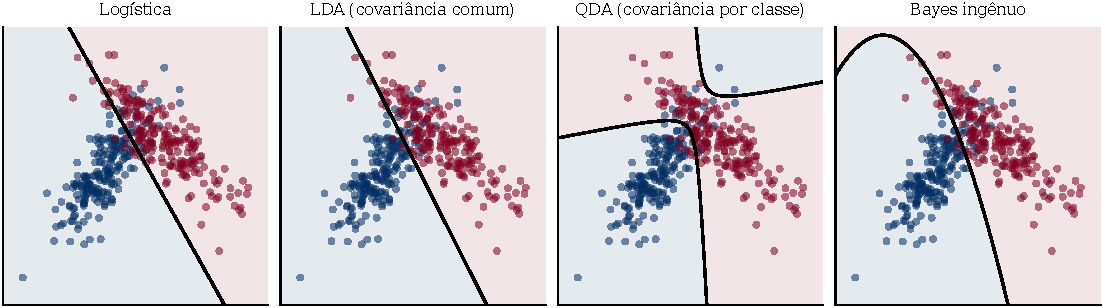
\includegraphics[width=\textwidth]{../../recursos/figuras/08-fronteiras.pdf}
  \caption{Fronteiras de decisão em duas classes gaussianas com covariâncias
  \emph{diferentes} ($n=400$). Logística e LDA chegam a retas quase idênticas por
  caminhos completamente distintos --- uma modelando $\Prob(Y\mid\x)$ direto, a
  outra modelando $f(\x\mid Y)$ e invertendo. O QDA, livre da hipótese de
  covariância comum, curva a fronteira e acompanha o formato de cada nuvem. O Bayes
  ingênuo também curva, mas erra o ângulo: ele supõe as duas covariáveis
  independentes dentro de cada classe, e aqui elas não são.}
  \label{fig:fronteiras}
\end{figure}

\subsection{LDA ou QDA? Uma questão de viés e variância}
QDA é mais flexível (menos viés) mas estima muito mais parâmetros. A conta: em $d$
dimensões, LDA estima \emph{uma} matriz de covariância, com $d(d+1)/2$ entradas
livres; QDA estima \emph{uma por classe}. Com $d=10$ e duas classes, são $55$
parâmetros contra $110$ --- e cada um deles precisa de dados.

\begin{figure}[htbp]
  \centering
  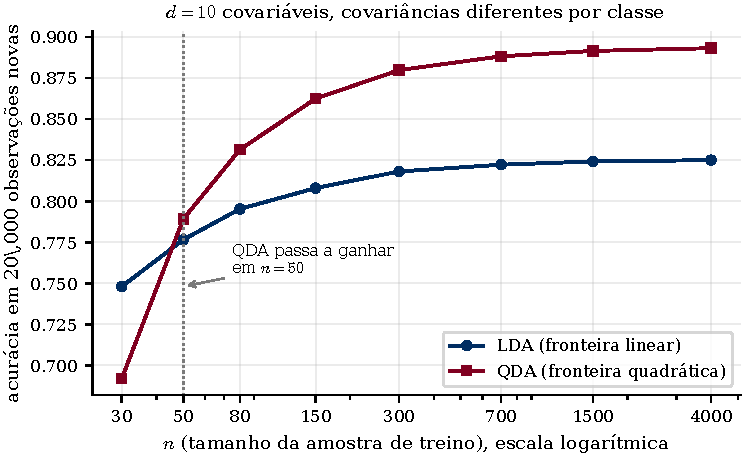
\includegraphics[width=0.72\textwidth]{../../recursos/figuras/08-lda-qda.pdf}
  \caption{Acurácia dos dois métodos em função de $n$, com $d=10$ covariáveis e
  covariâncias genuinamente diferentes por classe --- ou seja, num cenário em que o
  \textbf{QDA está certo e o LDA está errado}. Ainda assim, com $n=30$ o LDA ganha
  ($0{,}748$ contra $0{,}692$): não há dados para estimar $110$ parâmetros de
  covariância, e a variância do QDA supera o viés do LDA. A partir de $n=50$ o jogo
  vira, e em $n=4000$ o QDA abre sete pontos percentuais. Médias de 120 repetições,
  avaliadas em $20\,000$ observações novas.}
  \label{fig:ldaqda}
\end{figure}

\begin{ideia}
Esta figura é a Aula~01 vestida de classificação. O modelo \emph{correto} pode
perder para o modelo \emph{errado} quando não há dados suficientes para estimá-lo
--- exatamente o que o Exemplo~1.7 do [AME] mostrou lá atrás com polinômios de grau
5 e 2. Regra de bolso: LDA com poucos dados ou $d$ grande, QDA com muitos dados.
E, como sempre, valide de forma cruzada em vez de decidir por regra de bolso.
\end{ideia}

%==============================================================================
\section{Discriminativo $\times$ generativo}
%==============================================================================
\begin{center}\small
\renewcommand{\arraystretch}{1.3}
\begin{tabular}{@{}p{3.2cm}p{5.4cm}p{5.4cm}@{}}
\toprule
 & \textbf{Discriminativo (logística)} & \textbf{Generativo (LDA/QDA/NB)} \\
\midrule
Modela & $\Prob(Y\mid\x)$ direto & $f(\x\mid Y)$ e $\Prob(Y)$ \\
Suposições & poucas (forma do \emph{log-odds}) & distribucionais (gaussiana, indep.) \\
Quando brilha & muitos dados; suposições gaussianas falsas & classes bem separadas; poucos dados; suposições ~corretas \\
Bônus & --- & gera dados; lida com classes raras \\
\bottomrule
\end{tabular}
\end{center}

\begin{ideia}
Se as suposições gaussianas valem, LDA/QDA são (quase) ótimos e eficientes com
poucos dados. Se não valem, a logística --- que assume menos --- tende a ser mais
robusta com bastante dado. Um detalhe curioso fecha o círculo: sob as hipóteses do
LDA, o \emph{log-odds} sai \textbf{exatamente} linear em $\x$
(Prop.~\ref{prop:lda}), que é justamente o que a logística \eqref{eq:logit} supõe.
Os dois modelos coincidem em forma e diferem só em como estimam os coeficientes ---
o que explica os dois primeiros painéis da Figura~\ref{fig:fronteiras}. Na dúvida:
experimente ambos e compare por validação cruzada.
\end{ideia}

%==============================================================================
\section{Prática em Python}
%==============================================================================
\begin{lstlisting}
from sklearn.linear_model import LogisticRegression
from sklearn.discriminant_analysis import (LinearDiscriminantAnalysis as LDA,
                                           QuadraticDiscriminantAnalysis as QDA)
from sklearn.naive_bayes import GaussianNB
from sklearn.pipeline import make_pipeline
from sklearn.preprocessing import StandardScaler

# Logistica penalizada (C = 1/lambda); padronizar no pipeline (Aula 07)
logit = make_pipeline(StandardScaler(),
                      LogisticRegression(penalty="l2", C=1.0, max_iter=1000))

lda, qda, nb = LDA(), QDA(), GaussianNB()
for nome, modelo in [("logit", logit), ("LDA", lda), ("QDA", qda), ("NB", nb)]:
    modelo.fit(X_tr, y_tr)
    print(nome, "acuracia:", modelo.score(X_te, y_te))
    # probabilidades plug-in: modelo.predict_proba(X_te)
\end{lstlisting}

\begin{atencao}
Duas pegadinhas. Primeira: em \texttt{LogisticRegression}, o parâmetro é o
\texttt{C}, que é o \textbf{inverso} da penalização --- $C$ \emph{pequeno} significa
regularização \emph{forte}, ao contrário do \texttt{alpha} do Ridge/Lasso.
Segunda: \texttt{modelo.score} devolve \emph{acurácia}, e a caixa de atenção lá do
começo desta aula explica por que isso pode ser uma medida péssima. Leia a
Aula~09 antes de tirar conclusões dessas quatro linhas.
\end{atencao}

O notebook \texttt{Comparação entre classificadores paramétricos} confronta esses
métodos; \texttt{Aula prática 08} calcula o erro de Bayes numa população conhecida
e mede a troca LDA$\times$QDA em $d=2$ e $d=10$.

%==============================================================================
\section*{Resumo}
%==============================================================================
\begin{itemize}[leftmargin=1.4cm]
  \item Perda 0--1 \eqref{eq:risco01}; o \textbf{classificador de Bayes}
        $g^*(\x)=\argmax_c\Prob(Y=c\mid\x)$ é ótimo (Teo.~\ref{teo:bayes}) mas
        desconhecido --- é a moda condicional, como $r$ era a média condicional.
  \item \emph{Plug-in}: estimar $\Prob(Y=c\mid\x)$ e tomar o $\argmax$.
  \item \textbf{Logística} \eqref{eq:logit}: discriminativa, MV, penalizável,
        multinomial; respeita $[0,1]$; cuidado com separação perfeita.
  \item Generativos via Bayes \eqref{eq:gen}: \textbf{Bayes ingênuo} (indep.\
        condicional --- barata, mas descalibra), \textbf{LDA} (covariância comum
        $\to$ fronteira linear, Prop.~\ref{prop:lda}), \textbf{QDA} (covariância por
        classe $\to$ quadrática). Ver Fig.~\ref{fig:fronteiras}.
  \item LDA $\times$ QDA é viés $\times$ variância (Fig.~\ref{fig:ldaqda}): o
        modelo correto pode perder por falta de dados.
  \item Cuidado com acurácia em dados desbalanceados $\Rightarrow$ Aula~09.
\end{itemize}

\paragraph{Leitura recomendada.} [AME] Capítulo~7 (risco 0--1 e o classificador de
Bayes, com o Teorema~9 que é o nosso Teo.~\ref{teo:bayes}) e §8.1 (\emph{plug-in},
logística, Bayes ingênuo, LDA/QDA). [ISLP] Capítulo~4: §4.3 (logística, com a
interpretação dos coeficientes em razão de chances) e §4.4 (modelos generativos ---
a Figura~4.9 deles é a versão da nossa Figura~\ref{fig:fronteiras}, e §4.5 compara
todos os métodos num cenário simulado, complementando a nossa
Figura~\ref{fig:ldaqda}).

\paragraph{Para praticar.} \texttt{Lista teorica 08.pdf} (teórica, com gabarito) e \texttt{Lista prática 08.ipynb} (prática, para completar as lacunas), nesta mesma pasta.

\end{document}
